\documentclass[a4paper,11pt,twoside]{book}
\usepackage[DIV=14,BCOR=2mm,headinclude=true,footinclude=false]{typearea}
\usepackage[activate={true,nocompatibility},final,tracking=true,kerning=true,spacing=true,factor=1100,stretch=10,shrink=10]{microtype}
\usepackage[english]{babel}
\usepackage{enumerate}
\usepackage{longtable}
\usepackage{makecell}
\usepackage{comment}
\usepackage{tikz-feynman}
\usepackage{float}
\usepackage{graphicx}
\usepackage[format=plain,labelfont=it, textfont=it]{caption}
\usepackage{subcaption}
\usepackage{booktabs}
\usepackage{amsmath}
\usepackage{mathrsfs}
\usepackage{pgfplots}

\counterwithin{figure}{chapter} 
\counterwithin{equation}{section}

\newcommand{\de}[0]{\textrm{d}}



\usepackage[backend=bibtex,
style=numeric-comp, sorting=none, block=ragged, giveninits=true, ]{biblatex}
\addbibresource{mybiblio_2.bib}
\usepackage{hyperref}
\usepackage{cleveref}
\usepackage{graphicx}
\hypersetup{
colorlinks=true,
linkcolor=blue,
filecolor=magenta,
citecolor=red,
urlcolor=blue,
pdftitle={nico thesis},
pdfpagemode=FullScreen,
}



\setlength{\oddsidemargin}{8mm}   
\setlength{\textwidth}{145mm}     
\linespread{1.12}                


\renewcommand\labelitemi{\tiny$\bullet$}
\newcommand{\isotope}[2]{\textsuperscript{#1}#2}




\begin{document}
\pagenumbering{gobble}



\begin{titlepage}
	
\begin{figure}[H]
\centering

\includegraphics[width=360pt]{UniversitasMediolanensis.pdf}
\vspace{0.5 cm}
\end{figure}
	
	
\begin{center}{
Facoltà di scienze e tecnologie\\
Laurea Triennale in Fisica
}
\end{center}
	
\begin{center}
\vspace{1 cm}
{
\textbf{Separating the production of single top quarks in association with a Z boson from background events with Machine Learning techniques at the ATLAS experiment} }
\end{center}
\par
\vspace{2 cm}
	
\begin{flushleft}
Relatore:\\ \textbf{Lidia Dell'Asta}\\
\end{flushleft}
	
\vspace{1 cm}
\begin{flushright}
Tesi di Laurea Triennale di:\\ \textbf{Niccolò Laurora} \\Matricola: \textbf{932540}
\end{flushright}
	
\vfill
\begin{center}
{\large Anno Accademico 2021/2022}
\end{center}
\end{titlepage}



\cleardoublepage\thispagestyle{empty} 
\vspace*{1cm} 
\textit{
\flushright
alla mia famiglia
\vfill
}



\chapter*{\centering Abstract}






The study of the structures of molecular clouds is crucial not only because they play an important role in the mass of galaxies but also because they are the basis for the star formation process. \\

In the first and second chapters, I will provide an overview of molecular clouds and the methods used to study their density through the extinction of light. Specifically, I will discuss the star count method, NICE, NICER, and briefly touch on NICEST techniques.\\

In the third chapter, I will attempt to create some extinction maps related to the Orion Nebula using these techniques. \\

In the fourth and last chapter, I will present \textit{Dust} 1.0.0, an application developed by my advisor Marco Lombardi with the target to speed up and simplify the approach for the creation of the maps, implementing some boosted techniques, like XNICER and XNICEST, and I will use this application for making the extinction map with VISION data.



\newpage\null\thispagestyle{empty}\newpage
\tableofcontents
\newpage\null\thispagestyle{empty}\newpage

\pagenumbering{arabic}
\mainmatter

%primo capitolo
\chapter{Interstellar Medium}

\begin{figure}[H]
	\centering
	\includegraphics[width=\textwidth]{images/1_perseus_molecular_cloud.jpg}
	\caption{Perseus molecular cloud}
	\label{fig:image}
\end{figure}

Although most of the mass of the Milky Way Galaxy is considere into stars, intertellar space is not completely empty. It contains \textit{gas} and \textit{dust}.\\


The first clear evidence for the existence of interstellar dust was obtained around 1930. Before that, it had been generally thought that space is completely transparent and that light can propagate indefinitely without extinction. \\

In 1930 \textit{Robert Trumpler} published his study of the distribuction of the open clusters.
The absolute magnitudes M of the brightest stars could be estimated on the basis of the spectral type. Thus the distance r to the clusters could be calculated from the observed apparent magnitudes $m$ of the bright stars:
\begin{equation}
	m-M = 5\log{\frac{r}{10 \textrm{pc}}}
	\label{magnitude_distance}
\end{equation}
Trumpler also studied the diameters of the clusters. The linear diamenter $D$ is obtained from the apparent angular diameter $d$ by means of the formula 
\begin{equation}
	D=d\cdot r
\end{equation}
where $r$ is the distance of the clusters.\\

It caught Trumpler’s attention that the more distant clusters appeared to be systematically
larger than the nearer ones (\ref{fig:trumpler_cluster_distance}).\\

Since thiscould hardly be true, the distances of the more distant clusters must have been overestimated.\\
Trumpler concluded that the overestimation of distance in distant star clusters could not be true, and instead proposed that the dimming of starlight is due to some intervening material, thus showing \textbf{that space is not completely transparent}.

\begin{figure}[H]
	\centering
	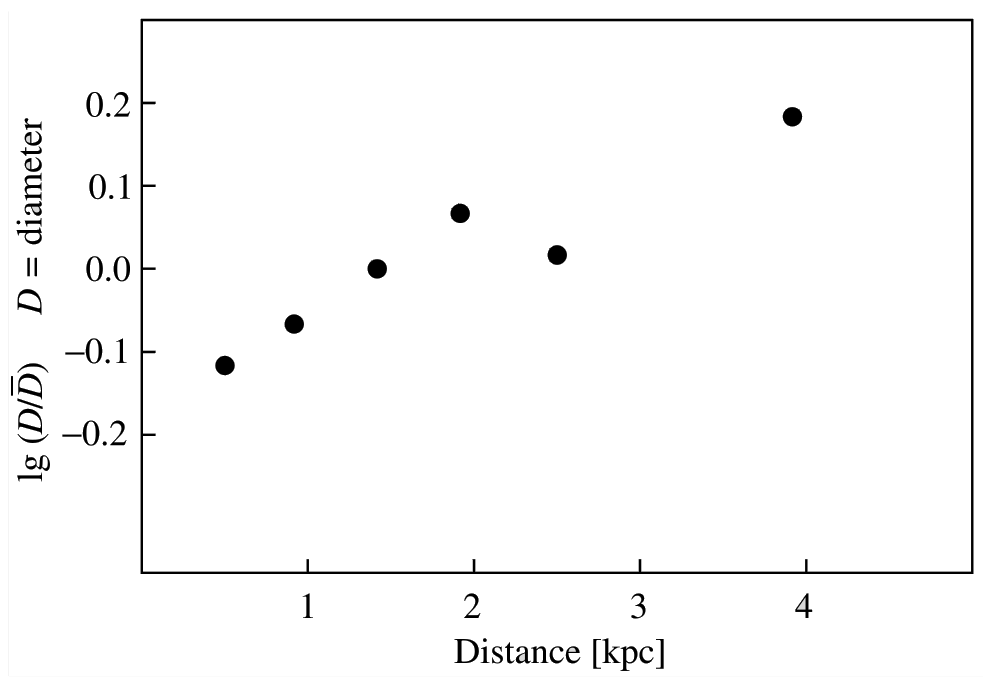
\includegraphics[width=0.7\linewidth]{images/trumpler_cluster_diameter.png}
	\caption{The increase in diameter of open star clusters with distance calculated by Trumpler (1930) is not a genuine trend, but rather a result of interstellar extinction, as discovered through the use of formula \eqref{magnitude_distance}.}
	\label{fig:trumpler_cluster_distance}
\end{figure}

To take this into account, \eqref{magnitude_distance} has to be replaced with an other formula.

\section{Extinction}

Equation \eqref{magnitude_distance} shows how the apparent magnitude increases (and brightness decreases!) with increasing distance. If the space between the radiation source and the observer is not completely empty, but contains some interstellar medium, \eqref{magnitude_distance} is not valid anymore beacuse \textit{part of the radiation is absorbed by the medium} (and usually re-emitted at a different wavelength, which may be outside the band defining the magnitude), or \textit{scattered away from the line of sight}. All these radiation losses are called the \textit{extinction}.\\

Now we want to find out how the extinction depends on the distance.\\

Assume we have a star radiating a flux $L_0$ into a solid angle $\omega$ in some wavelength range. Since the medium absorbs and scatters radiation, the flux $L$ will now decrease with increasing $r$.

\begin{figure}[H]
	\centering
	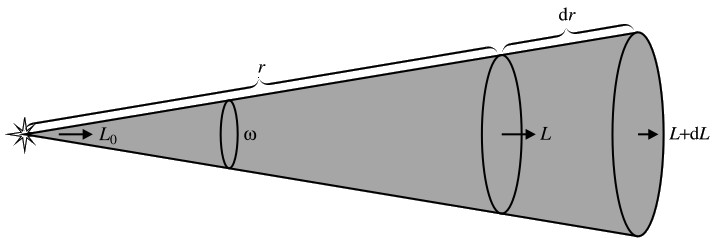
\includegraphics[width=0.7\linewidth]{images/interstellar_medium_absorbs.jpg}
	\caption{The interstellar
		medium absorbs and scatters radiation; this usually reduces the energy flux $L$ in the solid angle $\omega$}
	\label{fig:interstellar_medium_absorbs}
\end{figure}

In a short distance $[r, r+\de r]$, the extinction $\de L$ is proportional to the flux and the distance $L$ travelled in the medium: 
\begin{equation}
	\de L = -\alpha L \de r
	\label{eq:opacity}
\end{equation}

The factor $\alpha$ tells how effectively the medium can obscure the radiation. It is called \textit{opacity}. It approaches to zero for a perfect vacuum and to infinity when the substance becomes really murky.\\

We can define a dimensionaless quantity, the \textit{optical thickness} $\tau$ by 
\begin{equation}
	\de \tau = \alpha \de r
\end{equation}
Substituting this into \eqref{eq:opacity} we get
\begin{equation}
	\de L = - L \de \tau
\end{equation}
which, once integrated, becomes 
\begin{equation}
	L=L_0e^{-\tau}
	\label{eq:luminosity}
\end{equation}

Let $F_0$ be the flux density on the surface of a star and $F(r)$, the flux density at a distance $r$. We can express the fluxes as
\begin{equation}
	L=\omega r^2 F(r) \quad L_0=\omega R^2 F_0
\end{equation}
where $R$ is te radius of the star. Substitution into \eqref{eq:luminosity} gives
\begin{equation}
	F(r)=F_0\frac{R^2}{r^2}e^{-\tau}
\end{equation}
For the absolute magnitude we need the flux density at a distance of 10 parsecs, $F(10)$, which is still evaluated without extinction:
\begin{equation}
	F(10)=F_0\frac{R^2}{(10 \textrm{pc})^2}
\end{equation}
The distance modulus $m-M$ is now
\begin{align}
	m-M &= -2.5 \log{\frac{F(r)}{F(10)}} =\\
	& = 5 \log \frac{r}{10 \textrm{pc}} - 2.5 \log e^{-\tau} = \\
	& = 5 \log \frac{r}{10 \textrm{pc}} - (2.5 \log e)\tau
\end{align}
or
\begin{equation}
	m - M = 5\log \frac{r}{10 \textrm{pc}} + A
	\label{eq:magnitude_with_extinction}
\end{equation}
where $A\geq0$ is the extinction in magnitudes due to the entire medium between the star and the observer.\\

If the opacity is constant along the line of
sight, we have
\begin{equation}
	\tau = \alpha \int_0^r\de r = \alpha r 
\end{equation}
and the \eqref{eq:magnitude_with_extinction} becomes 

\begin{equation}
	m-M = 5\log \frac{r}{10 \textrm{pc}}+ar
\end{equation}

where the costant $a = 2.5\alpha \log e$ gives the extinction in magnitudes per unit distance. At present, a value of 2 mag/kpc is used for the average extinction. Thus the extinction over a 5 kpc path is already 10 magnitudes.\\

Extinction is due to dust grains that have diameters near the wavelength of the light.

\subsection{Absorption and scattering}

Interstellar particles can cause extinction in
two ways: 
\begin{itemize}
	\item In \textit{absorption} the radiant energy is transformed into heat, which is then re-radiated
	at infrared wavelengths corresponding to thetemperature of the dust particles.
	\item In \textit{scattering} the direction of light propagation
	is changed, leading to a reduced intensity in
	the original direction of propagation.
\end{itemize}

An expression for interstellar extinction will
now be derived.

\begin{figure}[H]
	\centering
	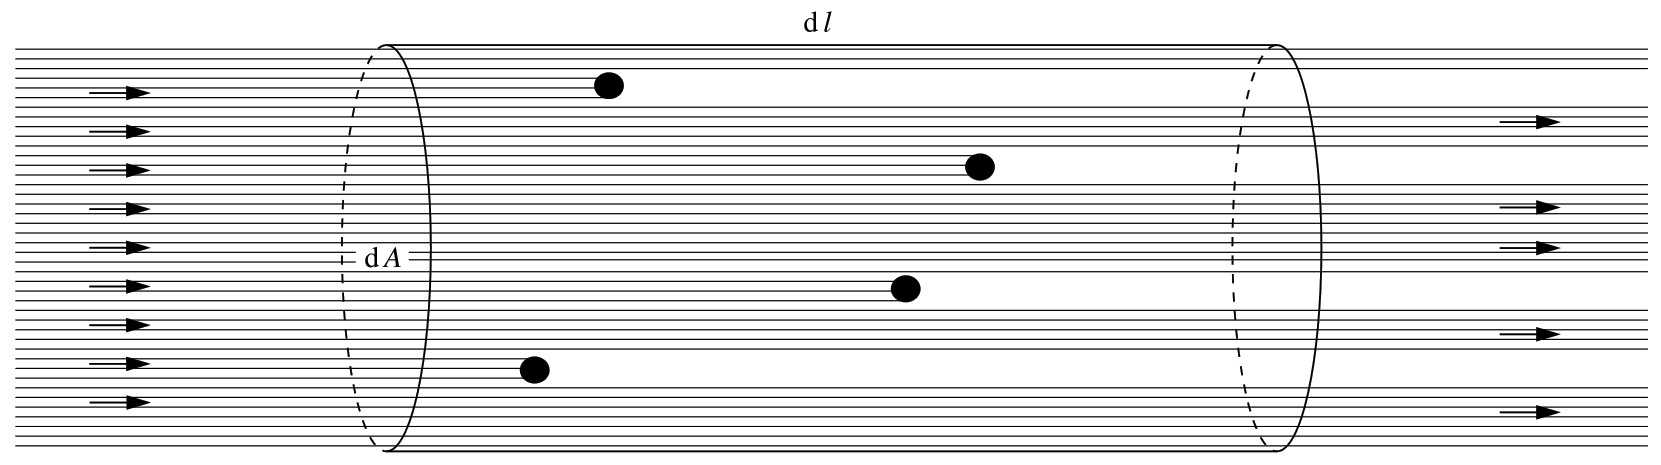
\includegraphics[width=\linewidth]{images/extinction_by_distribuction_of_particles.jpg}
	\caption{The interstellar
		mediuExtinction by a distribution of particles.}
	\label{fig:extinction_by_distribuction_of_particles}
\end{figure}

An expression for interstellar extinction will
now be derived. The size, index of refraction and number density of the particles are assumed to be known. For simplicity we shall assume that all
particles are spheres with the same radius $a$ and section $\pi a^2$. The true extinction cross section of the particles $C_\textrm{ext}$ will be

\begin{equation}
	C_\textrm{ext}=Q_\textrm{ext}\pi a^2
\end{equation}.

where $Q_{ext}$ is the extinction efficiency factor.

Let us consider a volume element with length
dl and cross section dA, normal to the direction
of propagation \ref{fig:interstellar_medium_absorbs}. It is assumed that the particles inside the element do not shadow each
other. If the particle density is $n$, there are $n\de l \de A$
particles in the volume element and they will
cover the fraction $\de \tau$ of the area $\de A$, where

\begin{equation}
	\de \tau = \frac{n \de A \de l C_\textrm{ext}}{\de A} = n C_\textrm{ext} \de l
\end{equation}
In the length $\de l$ the intensity is thus changed by
\begin{equation}
	\de I = - I \de \tau
\end{equation}

On the basis of \ref{fig:trumpler_cluster_distance} $\de \tau$ can be identified as the
optical depth.


The total optical depth between the star and the Earth is
\begin{equation}
	\tau(r) = \int_0^r\de \tau = \int_0^r nC_\textrm{ext}\de l = \overline{n}C_\textrm{ext}r
\end{equation}
where $\overline{n}$ is the average particle density along the
given path.

In accord to  \eqref{eq:magnitude_with_extinction} the extinction in
magnitudes is
\begin{equation}
	A = (2.5\log e )\tau
\end{equation}
and hence
\begin{equation}
	A = (2.5\log e )\overline{n}C_\textrm{ext}r
\end{equation}
This formula can also be inverted to calculate $\overline{n}$,
if the other quantities are known.
\
The extinction efficiency factor $Q_{\textrm{ext}}$ can be
calculated exactly for spherical particles with
given radius $a$ and refractive index $m$. In general,
\begin{equation}
	Q_\textrm{ext} = Q_\textrm{abs} +Q_\textrm{sca}
\end{equation}
If we define
\begin{equation}
	x = 2\pi a /\lambda
\end{equation}
where $\lambda$ is the wavelength of the radiation, then

\begin{equation}
		Q_\textrm{ext} = 	Q_\textrm{ext} (x,m)
\end{equation}


\begin{figure}[H]
	\centering
	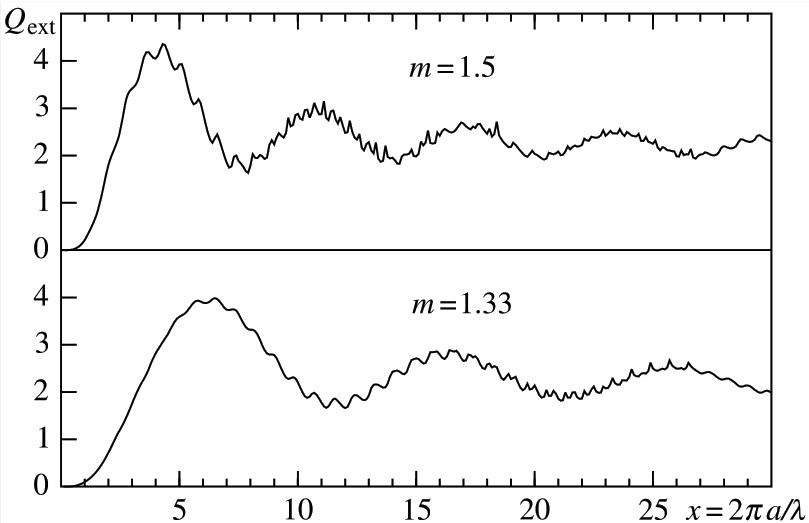
\includegraphics[width=\linewidth]{images/absorb_coefficient.jpg}
	\caption{Mie scattering: the extinction efficiency factor
		for spherical particles for the refractive indices $m = 1.5$
		and $m = 1.33$ (refractive index of water). The horizon-
		tal axis is related to the size of the particle according to
		$x = 2\pi a/\lambda$, where $a$ is the particle radius and $\lambda$, the wavelength of the radiation}
	\label{fig:absorb_coefficient}
\end{figure}

The exact expression for $Q_\textrm{ext}$ is a series ex-
pansion in x that converges more slowly for
larger values of $x$. When $x << 1$, the process is
called Rayleigh scattering; otherwise it is known as Mie scattering.

Figure \ref{fig:absorb_coefficient} shows $Q_\textrm{ext}$ as
a function of $x$ for $m = 1.5$ and $m = 1.33$. For
very large particles, $(x>>1)$ $Q_\textrm{ext}=2$, as appears
from \ref{fig:absorb_coefficient}. Purely geometrically one would
have expected $Q_\textrm{ext}=1$; the two times larger scat-
tering efficiency is due to the diffraction of light
at the edges of the particle.


\section{Reddening}

Another effect caused by the interstellar medium is the reddening of light: blue light is scattered and absorbed more than red.
Therefore the colour index $B-V$ increases.\\

The visual magnitude of a star is, from \eqref{eq:magnitude_with_extinction}
\begin{equation}
	V = M_V + 5 \log \frac{r}{10 \textrm{pc}}+ A_V
\end{equation}

where MV is the absolute visual magnitude and $A_V$ is the extinction in the $V$ passband. Similarly, we get for the blue magnitudes.

\begin{equation}
	B = M_B + 5 \log \frac{r}{10 \textrm{pc}}+ A_B
\end{equation}

The observed colour index is now
\begin{equation}
	B-V= M_B - M_V + A_B-A_V
\end{equation}
or

\begin{equation}
	B-V= (B - V)_0 + E_{B-V}
\end{equation}
where $(B-V)_0 = M_B - M_V $ is the \textit{instrinsec colour} of the star and $E_{B-V}=(B-V)-(B-V)_0$ is the \textit{colour excess}.\\

Studies of the interstellar medium show that the ratio of the visual extinction $A_V$ to the colour excess $E_{B-V}$ is almost
constant for all stars:

\begin{equation}
	R=\frac{A_V}{E_{B-V}} \approx 3.0
\end{equation}
This makes it possible to find the visual extinction
if the colour excess is known:
\begin{equation}
	A_V \approx 3.0 E_{B-V}
\end{equation}

Reddening is due to the fact that that the amount of extinction becomes larger for shorter wavelengths. Going from red to ultraviolet, the extinction is roughly inversely proportional to wavelength. For this reason \textit{the light of distant stars is redder than would be expected on
the basis of their spectral class}.

\subsection{Reddeing in function of the wavelegnth}
The wavelength dependence of the extinction, $A(\lambda)$, can be studied by comparing the magnitudes of stars of the same spectral class in different colours.\\

These measurements have shown that $A(\lambda)$ approaches zero as $\lambda$ becomes very large. As show in \ref{fig:barnard_68_at_different_wls} the extinction decreases with the increasing of wavelegnth. In practice $A(\lambda)$ can be measured up to a wavelength of about two micrometres.

\begin{figure}[H]
	\centering
	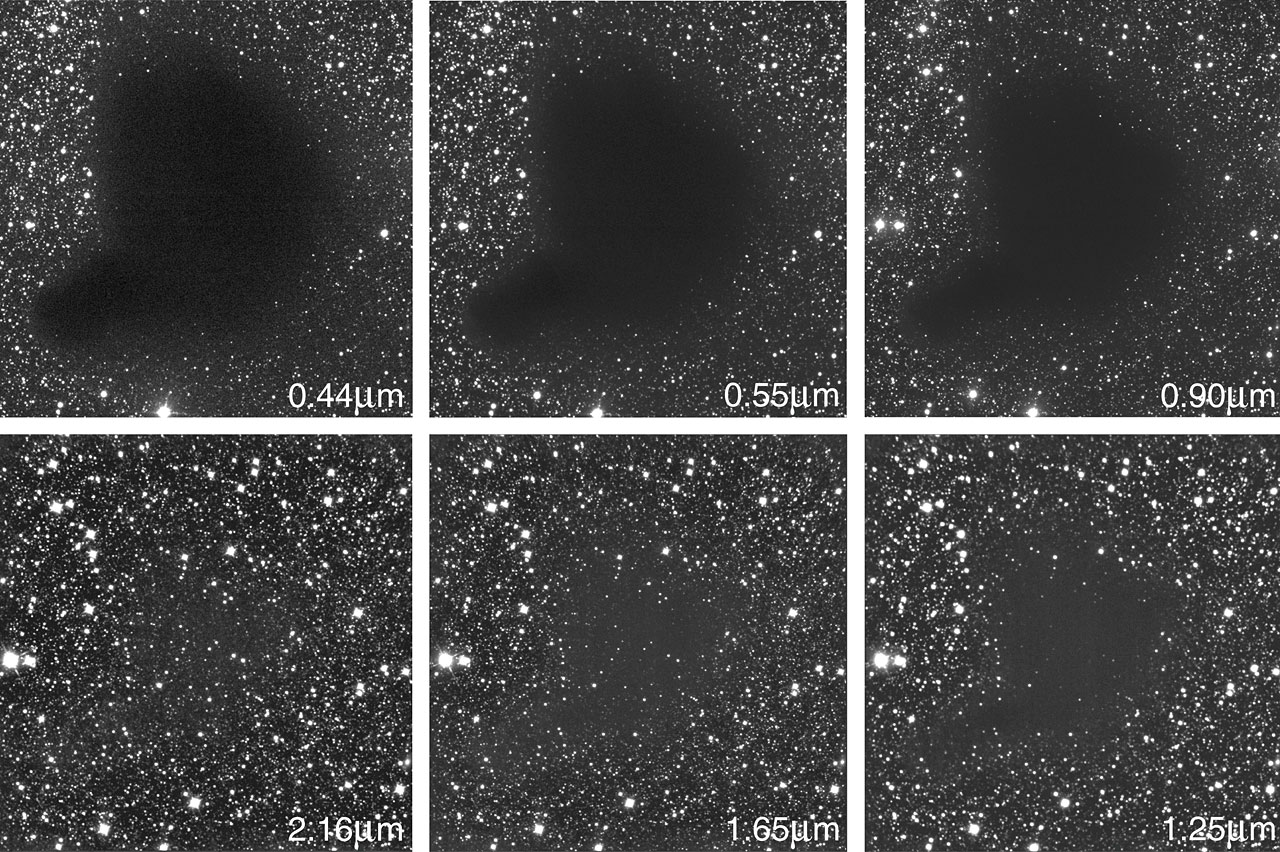
\includegraphics[width=\linewidth]{images/barnard_68.jpg}
		\caption{This image represents the sky area of the so-called Bok globule Barnard 68. It is evident that the obscuration caused by the cloud diminishes dramatically with increasing wavelength. Since the outer regions of the cloud are less dense than the inner ones, the apparent size of the cloud also decreases, as more background stars shine through the outer parts.
		Credit: ESO}
	\label{fig:barnard_68_at_different_wls}
\end{figure}

Hence, we can extrapolate the \textit{reddening curve} in figure \ref{fig:reddening_curve}:

\begin{figure}[H]
	\centering
	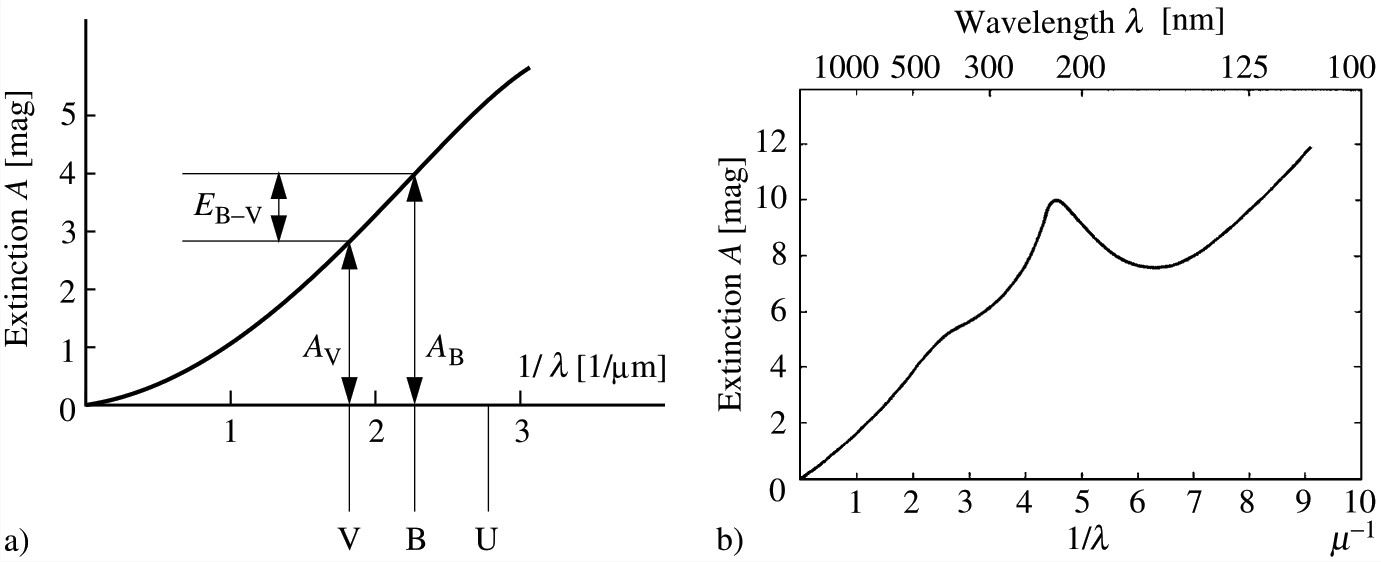
\includegraphics[width=\linewidth]{images/reddening_curve.jpg}
	\caption{a) Schematic representation of the interstellar extinction. As the wavelength increases, the extinction approaches zero. b) Measured extinction curve,
		normalised to make $E_{B-V} = 1$.
		Credit: Fundamental Astronomy book}
	\label{fig:reddening_curve}
\end{figure}




%secondo capitolo
\chapter{Methods for the determination of Extinction}

\section{Star Count}
In order to determinate the extinction A, a possible method is to count the number of the stars in a field. Suppose we have an exposure with threshold magnitude $m_0$. If extinction is present, we only see stars with magnitude 
\begin{equation}
	m < m_0 - A
\end{equation}

Let's define a "luminosity function" of observed stars $N'(m)$ so that:
\begin{equation}
	N'(m)\de m
\end{equation}
is the number of stars ranging from $m$ and $m+\de m$.

At this point, we need to choose two regions: the \textit{Control field}, where we suppose extinction is not present, and the \textit{Science field}, the zone where we assume extinction is present.\\

Now we count the number of stars $N_1$ in the control field and $N_2$ in the science field:
\begin{equation}
	N_1(m_0) = \int_{\infty}^{m_0} N'(m')\de m'
\end{equation}
\begin{equation}
	N_2(m_0-A) = \int_{\infty}^{m_0-A} N'(m')\de m'
\end{equation}

In the hypotesis that $N'(m)$ is the same for both fields, i can get the value of $A$.
\begin{center}
	\begin{tikzpicture}
		\begin{axis}[
			xlabel={$m$},
			ylabel={$\log N'(m)$},
			axis lines=left,
			xmin=0,
			ymin=0,
			xtick=\empty, % remove x tick marks and labels
			ytick=\empty, % remove y tick marks and labels
			]
			\addplot[domain=0:6,blue,thick]{(x-1)};
			\addplot[domain=0:11,red,thick]{(x-6)};
			\legend{control,science}
			
			% add arrow with label
			\draw[->,>=stealth,decorate,decoration={markings,mark=at position 0.5 with {\node[above]{$A$};}}] (axis cs:3,2) -- (axis cs:3,-3);
			
		\end{axis}
	\end{tikzpicture}
\end{center}





%terzo capitolo
\chapter{Analysis and Maps Production}



%quarto capitolo
\chapter{New Application for Analysis: Dust}


%quinto capitolo
%\chapter{Separation of tZq from background with DNNs} 



\backmatter
\addcontentsline{toc}{chapter}{Bibliography}

\printbibliography
\end{document}

